\documentclass[aspectratio=169]{beamer}
	\usepackage[utf8]{inputenc}		% Required for umlauts
	\usepackage[english]{babel}		% Language
	%\usepackage[sfdefault]{roboto}	% Enable sans serif font roboto
	%\usepackage{libertine}			% Enable this on Windows to allow for microtype
	\usepackage[T1]{fontenc}		% Required for output of umlauts in PDF

	\usepackage{mathtools}		% Required for formulas

	\usepackage{caption}		% Customize caption aesthetics
	\usepackage{tcolorbox}		% Fancy colored boxes
	\usepackage{xcolor}			% Highlighting
	\usepackage{soul}

	\usepackage{booktabs}		% Using pandas' LaTeX output
	\usepackage{multirow}		% Enable fancy table structure

	\usepackage{listings}		% Insert programming code
	\usepackage{graphicx}		% Required to insert images
	\usepackage{subcaption}		% Enable sub-figure
	\usepackage[space]{grffile} % Insert images baring a filename which contains spaces
	\usepackage{float}			% Allow to forcefully set the location of an object

	\usepackage[tracking=true]{microtype} % Required to change character spacing

	\usepackage[style=alphabetic,backend=biber,sorting=none,giveninits=true,isbn=false,url=false]{biblatex}
	\usepackage{csquotes}		% Ensure proper quotation of texts with babel and polyglossia with biblatex
	\usepackage{hyperref}		% Insert clickable references

	\usepackage{datetime}		% Flexible date specification
	\newcommand{\leadingzero}[1]{\ifnum#1<10 0\the#1\else\the#1\fi}
	\newcommand{\todayddmmyyyy}{\leadingzero{\day}.\leadingzero{\month}.\the\year}
	\newcommand{\mathcolorbox}[2]{\colorbox{#1}{$\displaystyle #2$}}

	\usepackage{geometry}
	\usepackage{scrextend}		% Allow arbitrary indentation

	\usepackage{color}

	\usepackage{appendixnumberbeamer}	% Fancy page numbering excluding the appendix

	% Compile notes into a separate file readable by pdfpc using a custom package which overwrite the `note` macro
	\usepackage{../pdfpcnotes}

	\makeatletter
	% Fix subfig in beamer style presentation
	\let\@@magyar@captionfix\relax

	% Insert [short title] for \section in ToC
	\patchcmd{\beamer@section}{{#2}{\the\c@page}}{{#1}{\the\c@page}}{}{}
	% Insert [short title] for \section in Navigation
	\patchcmd{\beamer@section}{{\the\c@section}{\secname}}{{\the\c@section}{#1}}{}{}
	% Insert [short title] for \subsection in ToC
	\patchcmd{\beamer@subsection}{{#2}{\the\c@page}}{{#1}{\the\c@page}}{}{}
	% Insert [short title] for \subsection in Navigation
	\patchcmd{\beamer@subsection}{{\the\c@subsection}{#2}}{{\the\c@subsection}{#1}}{}{}
	\makeatother

	\addbibresource{../literature.bib}

	\setbeamercolor{title}{fg=orange}
	\setbeamertemplate{title}{
		\color{orange}
		\textbf{\inserttitle}
	}
	\setbeamercolor{tableofcontents}{fg=orange}
	\setbeamercolor{section in toc}{fg=black}
	\setbeamercolor{subsection in toc}{fg=black}
	\setbeamertemplate{frametitle}{
		%\vspace{0.5em}
		\color{orange}
		\begin{center}
			\textbf{\insertframetitle} \\
			{\small \insertframesubtitle}
		\end{center}
	}
	\setbeamertemplate{footline}[text line]{
		\parbox{\linewidth}{
			\color{gray}
			\vspace*{-1em}
			NII 2018
			\hfill
			Gordian (\href{mailto:gordian.edenhofer@gmail.com}{gordian.edenhofer@gmail.com})
			\hfill
			\insertframenumber/\inserttotalframenumber%
		}
	}
	\setbeamertemplate{navigation symbols}{}
	\setbeamertemplate{itemize item}{\color{black}$\bullet$}
	\setbeamertemplate{itemize subitem}{\color{black}$\circ$}
	\setbeamercolor{block title}{fg=black}
	\captionsetup{font=scriptsize,labelfont={bf,scriptsize}}

	\lstset{basicstyle=\ttfamily,breaklines=true,showstringspaces=false,commentstyle=\color{red},keywordstyle=\color{blue}}

	\title{Augmenting the DonorsChoose.org Corpus for Meta-Learning}
	\subtitle{``Meta-Learning for Recommender Systems''}
	\author[Edenhofer]{\href{mailto:gordian.edenhofer@gmail.com}{Gordian Edenhofer}}
	\institute[NII]{
		Working Group of Prof.~Dr.~Beel, Trinity College Dublin \\
		Laboratory of Prof.~Dr.~Akiko~Aizawa, Nationa Institute of Informatics
	}
	\date[Research Internship 2018]{National Institute of Informatics, \formatdate{09}{10}{2018}}
	\subject{Natural Language Processing and Machine Translation}


\begin{document}

\pagenumbering{arabic}

\begin{frame}[plain,noframenumbering]
	\titlepage%
\end{frame}

\section[Introduction]{Research Problem}
\frame{\vfill\centering\tableofcontents[sectionstyle=show/shaded,subsectionstyle=show/hide]\vfill}

\subsection{Lack of Datasets}
\begin{frame}
	\frametitle{\insertsection}
	\framesubtitle{\insertsubsection}

	\begin{itemize}
		\item Meta-learning for recommender systems
		\begin{itemize}
			\item Combine strengths of individual learners
			\item Incorporate more transaction details
		\end{itemize}
		\item Absence of datasets with metadata
		\begin{itemize}
			\item Time-consuming and cumbersome to construct and implement learning subsystem
			\item Drains resources from actual meta-learning experiment
			\item Manual augmentation is often redundant~\cite{CUNHA2018128,DBLP:journals/corr/abs-1805-12118,Ekstrand:2012:RFP:2365952.2366002}
			\note{Redundant manual augmentation: 5 out of 7 reviewed meta-learners use MovieLense data}
		\end{itemize}
	\end{itemize}
\end{frame}

\subsection{Augmenting DonorsChoose.org}
\begin{frame}
	\frametitle{\insertsection}
	\framesubtitle{\insertsubsection}

	\begin{itemize}
		\item Publish augmented dataset
		\begin{itemize}
			\item Find dataset suitable for meta-learning with sufficient user-, item- and transaction-information
			\item Add metadata of single recommender algorithms, statistics, etc.~to the dataset
		\end{itemize}
		\item Encourage evaluation of meta-learner experiments on this dataset
	\end{itemize}
\end{frame}

\section[Methodology]{Augmentation}
\frame{\vfill\centering\tableofcontents[sectionstyle=show/shaded,subsectionstyle=show/hide]\vfill}

\subsection{The DonorsChoose.org Dataset}
\begin{frame}
	\frametitle{\insertsection}
	\framesubtitle{\insertsubsection}

	\begin{itemize}
		\item DonorsChoose.org transaction dataset
		\begin{itemize}
			\item \$686 million raised
			\item 4,69 million transactions (donations); 2,12 million users (donors); 1,11 million items (projects)
		\end{itemize}
		\item Available features
		\begin{itemize}
			\item User: location, teacher status
			\item Item: location, category, descriptions, funding goals, creator
			\item Transaction: strength (donated amount), time
		\end{itemize}
		\item Amendments
		\begin{itemize}
			\item Learning Subsystem: Two collaborative, two content-based recommender algorithms
			\item Statistics: Aggregated user and item statistics
			\item Exemplary Meta-Learners: Algorithm Selection Problem via stacking hybrid ensemble
		\end{itemize}
	\end{itemize}
\end{frame}

\begin{frame}
	\frametitle{\insertsection}
	\framesubtitle{\insertsubsection}

	\begin{figure}
		\centering
		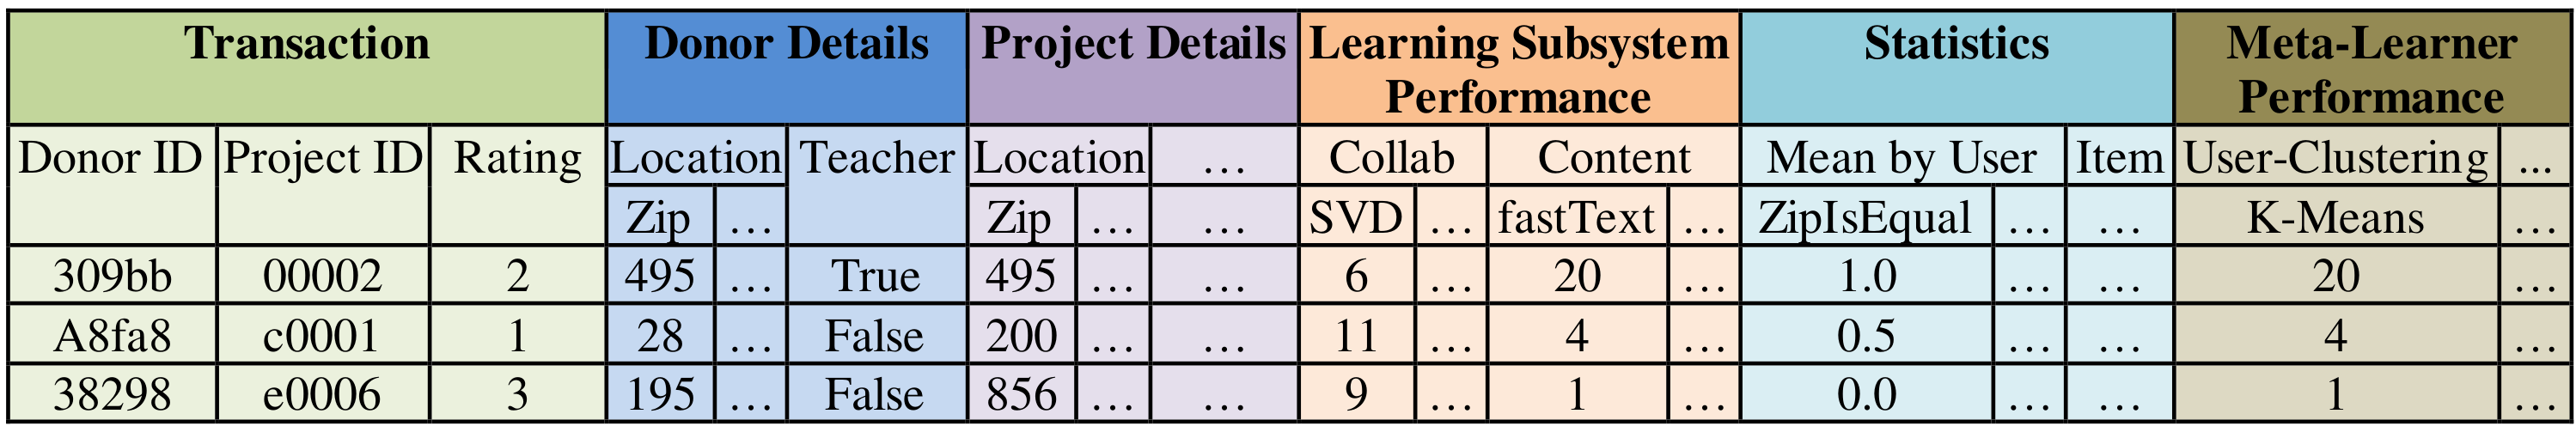
\includegraphics[width=\textwidth,height=0.6\textheight,keepaspectratio]{{{../res/Illustrative example of the overall design of the augmented transaction table}}}
		\caption{Illustrative example of the overall design of the augmented transaction table with
		amended learning subsystem performance scores, statistics and meta-learner information.}
	\end{figure}
\end{frame}

\subsection{Dataset Preparation}
\begin{frame}
	\frametitle{\insertsection}
	\framesubtitle{\insertsubsection}

	\begin{itemize}
		\item House keeping
		\begin{itemize}
			\item Merging duplicate transaction
			\item Remove stop-words
			\item Drop transactions with NaN as location
		\end{itemize}
		\item Enforced Requirements
		\begin{itemize}
			\item Users having donated at least twice for training and testing
			\item No transactions of \$2 or below as low user-interest assumed
		\end{itemize}
		\item Transformation
		\begin{itemize}
			\item DonationAmount to interaction strength
			\item Sampling 100,000 transaction
		\end{itemize}
	\end{itemize}
\end{frame}

\subsection{Learning Subsystem}
\begin{frame}
	\frametitle{\insertsection}
	\framesubtitle{\insertsubsection}

	\begin{itemize}
		\item Cross-validation using $5$ folds
		\item Top-N accuracy using the recall~\cite{Cremonesi:2010:PRA:1864708.1864721}
		\begin{itemize}
			\item Randomized subset of $100$ projects the user has not donated to
			\item One project to which the user has donated to
			\item Recall@N is predicted position of donated project in the subset of $101$ projects
		\end{itemize}
	\end{itemize}

	\begin{table}
		\scriptsize
		\centering
		\begin{tabular}{l|lll}
			Filtering method & Algorithm & Computational method & Yields \\
			\hline
			\hline
			collaborative & KNN & neirest-neighbor (2-norm) & RMSE, MAE, \colorbox{yellow}{Recall@N} \\
			& SVD & matrix factorization & RMSE, MAE, \colorbox{yellow}{Recall@N} \\
			\hline
			content-based & TF-IDF & term frequency & cosine similarity, \colorbox{yellow}{Recall@N} \\
			\hline
			content-based, neural network & fastText & word-embedding & cosine similarity, \colorbox{yellow}{Recall@N} \\
		\end{tabular}
		\caption{Architecture of the learning subsystem with a list of properties for each algorithm.}
	\end{table}
\end{frame}

\subsection{Statistics and Application of Learning Subsystem}
\begin{frame}
	\frametitle{\insertsection}
	\framesubtitle{\insertsubsection}

	\begin{itemize}
		\item Holdout-validation using $80\%$ train-test-split
		\item Statistics
		\begin{itemize}
			\item Aggregated user information on value counts for past donations
			\item Aggregated item location, category, etc.~information grouped by user
		\end{itemize}
		\item Meta-learner approaches
		\begin{itemize}
			\item Transaction classification via a decision tree
			\item Error prediction using gradient boosting
			\item User-clustering using K-Means
			\item Stacking decision tree as classifier
		\end{itemize}
	\end{itemize}
\end{frame}

\section[Results]{Augmented Corpus}
\frame{\vfill\centering\tableofcontents[sectionstyle=show/shaded,subsectionstyle=show/hide]\vfill}

\subsection{Shape}
\begin{frame}
	\frametitle{\insertsection}
	\framesubtitle{\insertsubsection}

	\begin{itemize}
		\item More than half of transactions preserved ($>>$ sample size)
		\item Sample of 100,000 transactions: 21,087 unique users and 91,827 unique projects
	\end{itemize}

	\begin{figure}[ht]
		\centering
		\subcaptionbox{Transactions per user\label{fig:dist_number_of_interactions_per_user}}{
			\includegraphics[width=0.35\textwidth,height=\textheight,keepaspectratio]{{{../res/DonorID - Distribution of number of interactions per user}}}
		}
		\hspace{2em}
		\subcaptionbox{Ratings\label{fig:dist_transaformed_ratings}}{
			\includegraphics[width=0.35\textwidth,height=\textheight,keepaspectratio]{{{../res/DonationAmount - Distribution of ratings for logarithmic bins and excluded outliers}}}
		}
		\caption{Distribution of the number of transactions per user and the rating scores to which the donated amount has been transformed to.}
		\label{fig:dataset_sample_dist}
	\end{figure}
\end{frame}

\subsection{Learning Subsystem}
\begin{frame}
	\frametitle{\insertsection}
	\framesubtitle{\insertsubsection}

	\begin{figure}
		\centering
		\includegraphics[width=\textwidth,height=0.6\textheight,keepaspectratio]{{{../res/Learning subsystem - Position in Top-N test set}}}
		\caption{Statistical features of the distribution of the donated item position in the Recall@N test set. The dashed orange line indicates the median, the green line the mean.}
	\end{figure}
\end{frame}

\subsection{Exemplary Meta-Learning Experiment}
\begin{frame}
	\frametitle{\insertsection}
	\framesubtitle{\insertsubsection}

	\begin{figure}
		\centering
		\includegraphics[width=\textwidth,height=0.6\textheight,keepaspectratio]{{{../res/Meta-learner Performance - Average position in Top-N test set for various meta-learner algorithms with augmented learning subsystem filtering techniques}}}
		\caption{Performance of the four meta-learners in comparison to the overall best algorithm.}
	\end{figure}
\end{frame}

\section{Conclusion}
\frame{\vfill\centering\tableofcontents[sectionstyle=show/shaded,subsectionstyle=show/hide]\vfill}

\subsection{Extensively Augmented DonorsChoose.org Dataset}
\begin{frame}
	\frametitle{\insertsection}
	\framesubtitle{\insertsubsection}

	\begin{itemize}
		\item Feature-rich and big corpus
		\item Extensively augmented features
		\begin{itemize}
			\item Learning subsystem
			\item Aggregated user and transaction statistics
			\item Limited success in solving the Algorithm Selection Problem via switching hybrid ensemble
		\end{itemize}
		{
			\setbeamertemplate{itemize item}{\color{black}$\Rightarrow$}
			\item Excellent candidate for further meta-learning experiments
		}
	\end{itemize}
\end{frame}

\appendix

\begin{frame}[shrink=20]
	\frametitle{Bibliography}

	\printbibliography%
\end{frame}

\end{document}
